\chapter{Croissant Appendix}

\section{FMTI}

\textbf{Disclaimers and Methodology} 

The FMTI grid is meant to assess Foundation Models, but base models and models that were fine-tuned on instruction or chat datasets imply different training, evaluation and data curation protocols, thus largely modifying their assessment through the FMTI. Training an instruction or chat model from a base model is a process that has recently been completely democratized through the use of crowdsourced or synthetic datasets, and individuals are now fully capable of finetuning their own model variants in a variety of manners. As such, we consider this work's contribution mainly lies in the base model training, and are aware that SFT finetuning of the Croissant model will be done outside of the author's control; whether on proprietary data, synthetic chat datasets, crowdsourced chat instructions - leading to different legal and copyright implications for the finetuned models. We thus focus on the base model in our evaluation and give the complete criteria list as detailed in the appendix. 

Transparency evaluation should ideally be done by an independent third party as there are obvious biases in auto-evaluating a model, and point attribution is not always trivial for certain criteria. As such, we take a rather conservative approach to point attribution and detail our process in an open document. Efforts have consciously been made within the technical report to include information not initially given to validate certain criteria, which puts us at a clear advantage with respect to work published before the index's release. 

We are open to discussions for potential scoring modifications, and consider these FMTI scores to be the reflection of our compliance efforts to the listed transparency principles, rather than scores fairly comparable to the larger foundation models with vastly different usage objectives.


\begin{figure}
    % First figure
    \centering
    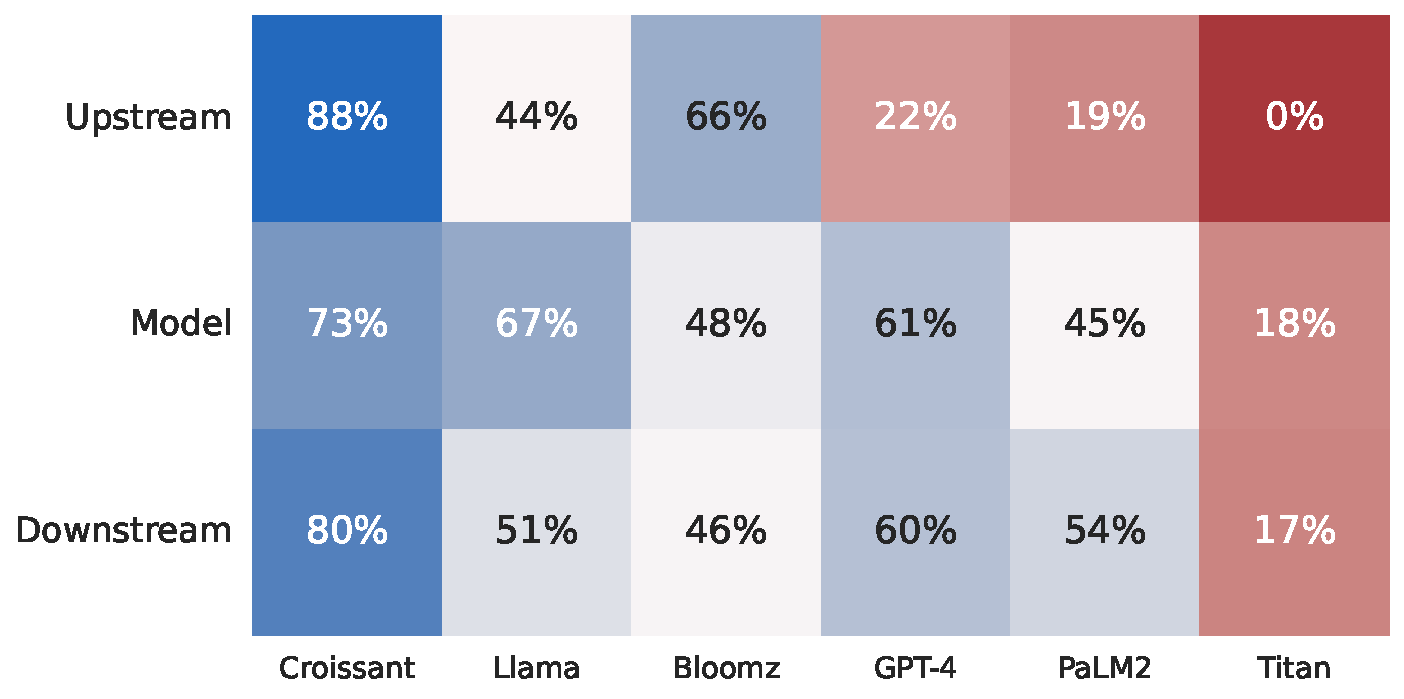
\includegraphics[width=\textwidth]{images/croissant_images/FMTI_heatmap_2.pdf}
    \caption[Aggregated FMTI]{Aggregated FMTI}
    \label{fig:fmti2}
\end{figure}



\newpage
\section{Additional data details}
\label{sec:appendix}

\subsection{French Data}
Refer to Table~\ref{tab:tab_fr}.

\begin{table*}
    \centering
        \begin{tabular}{lllll}
        \toprule
        Dataset & Size (GB) & Documents & Tokens (M) & Token/Doc \\
        \midrule
        CulturaxFr & 1216.03 & 363197906 & 292833.75 & 806.14 \\
        WikisourceFr & 10.84 & 2557238 & 2699.00 & 1055.44 \\
        Wikipedia20231101.fr & 7.37 & 2563646 & 2002.51 & 781.12 \\
        JadeOpendata & 5.19 & 550065 & 1295.29 & 2354.79 \\
        JorfOpendata & 3.83 & 3189949 & 967.10 & 303.17 \\
        LegiOpendata & 3.56 & 2151510 & 816.44 & 379.47 \\
        AccoOpendata & 3.39 & 251332 & 758.15 & 3016.52 \\
        IncaOpendata & 2.60 & 369687 & 627.32 & 1696.90 \\
        ProjectgutenbergFr & 0.97 & 2447 & 301.19 & 123086.16 \\
        CappOpendata & 0.91 & 71949 & 247.14 & 3434.97 \\
        CustomLayoutDatasetTextOnly & 0.77 & 291604 & 191.11 & 655.38 \\
        DebatsOpendata & 0.77 & 2114 & 149.09 & 70524.31 \\
        CassOpendata & 0.76 & 140803 & 206.04 & 1463.35 \\
        KaliOpendata & 0.68 & 402963 & 152.33 & 378.01 \\
        SwissLegislation & 0.26 & 11086 & 68.33 & 6163.81 \\
        FrenchOpenSubtitles & 0.15 & 5379 & 41.84 & 7779.26 \\
        CnilOpendata & 0.12 & 15168 & 26.37 & 1738.72 \\
        BnfClean2023 & 0.10 & 341 & 27.04 & 79295.71 \\
        QrOpendata & 0.10 & 530 & 21.73 & 41005.03 \\
        SardeOpendata & 0.09 & 221278 & 28.10 & 127.01 \\
        DoleOpendata & 0.08 & 4000 & 19.36 & 4839.07 \\
        ConstitOpendata & 0.07 & 6977 & 15.27 & 2188.28 \\
        FrenchLibrispeechTextOnly & 0.06 & 255631 & 12.91 & 50.49 \\
        FrenchPodcasts & 0.01 & 1237 & 1.56 & 1259.90 \\
        FrenchPoetry & 0.00 & 1721 & 0.76 & 441.23 \\
        \hline
        Train & 1258.70 & 376266561 & 303509.73 & 806.63 \\
        \bottomrule
        \end{tabular}
    \caption[French data mix]{French Data mix}
    \label{tab:tab_fr}
\end{table*}

\subsection{English data}

Refer to Table~\ref{tab:tab_en}.
\begin{table*}
    \centering
\begin{tabular}{lllll}
    \toprule
    Dataset & Size (GB) & Documents & Tokens (M) & Token/Doc \\
    \midrule
    SlimPajama & 2333.77 & 590194779 & 630441.67 & 1068.19 \\
    Project Gutenberg PG19 & 10.67 & 28602 & 23580.49 & 824435.00 \\
    Gutenberg Canaries & 2.75 & 7515 & 555.40 & 73905.01 \\
    \midrule
    Train & 2351.13 & 591230543 & 655637.48 & 1108.94 \\
    \bottomrule
    \end{tabular}
    
    \caption[English data mix]{English Data mix}
    \label{tab:tab_en}
\end{table*}


\subsection{Code data}
Refer to Table~\ref{tab:tab_code}.

\begin{table*}
    \centering
        \begin{tabular}{lllll}
        \toprule
        Dataset & Size (GB) & Documents & Tokens (M) & Token/Doc \\
        \midrule
        StarcoderdataJava & 82.49 & 20061773 & 29740.73 & 1482.46 \\
        StarcoderdataJavascript & 61.64 & 19534285 & 24546.60 & 1256.59 \\
        StarcoderdataPython & 57.00 & 12856649 & 24605.09 & 1913.80 \\
        StarcoderdataC & 50.60 & 8526791 & 15791.76 & 1852.02 \\
        StarcoderdataCpp & 45.84 & 6343527 & 19607.90 & 3091.01 \\
        PypiClean & 29.20 & 2428172 & 12120.74 & 4991.72 \\
        StarcoderdataSql & 10.38 & 965666 & 3278.24 & 3394.80 \\
        StarcoderdataJupyterScriptsDedupFiltered & 6.67 & 905365 & 2567.77 & 2836.18 \\
        StarcoderdataJupyterStructuredCleanDedup & 5.55 & 662056 & 2119.72 & 3201.72 \\
        StarcoderdataJson & 5.43 & 4741547 & 2165.87 & 456.79 \\
        StarcoderdataTex & 4.86 & 517551 & 1916.88 & 3703.76 \\
        StarcoderdataShell & 2.98 & 2196327 & 1178.17 & 536.43 \\
        CodeContests & 2.79 & 1485888 & 1228.61 & 826.85 \\
        StarcoderdataCuda & 0.52 & 57570 & 227.24 & 3947.14 \\
        GithubJupyterCodeToText & 0.48 & 46978 & 159.49 & 3395.09 \\
        StarcoderdataDockerfile & 0.41 & 565791 & 161.48 & 285.41 \\
        StarcoderdataIdris & 0.03 & 7942 & 11.72 & 1475.09 \\
        \hline
        Train & 366.87 & 81903878 & 141428.02 & 1726.76 \\
        \bottomrule
        \end{tabular}

    \caption[Code data mix]{Code Data mix}
    \label{tab:tab_code}
\end{table*}


\subsection{Parallel data}
Refer to Table~\ref{tab:tab_al}.
\begin{table*}
    \centering
        \begin{tabular}{lllll}
        \toprule
        Dataset & Size (GB) & Documents & Tokens (M) & Token/Doc \\
        \midrule
        CustomFrEn & 113.35 & 407858836 & 35641.60 & 87.39 \\
        ThesesFr20132023 & 0.36 & 95009 & 81.60 & 858.91 \\
        OriginalSongsLyricsWithFrenchTranslation & 0.20 & 75020 & 53.48 & 712.93 \\
        \hline
        Train & 113.91 & 408028865 & 35776.69 & 87.68 \\
        \bottomrule
        \end{tabular}

    \caption[Parallel data mix]{Parallel Data mix}
    \label{tab:tab_al}
\end{table*}

OPUS data distribution is given in Figure \ref{fig:opus}.

\begin{figure}[ht]
    \centering
    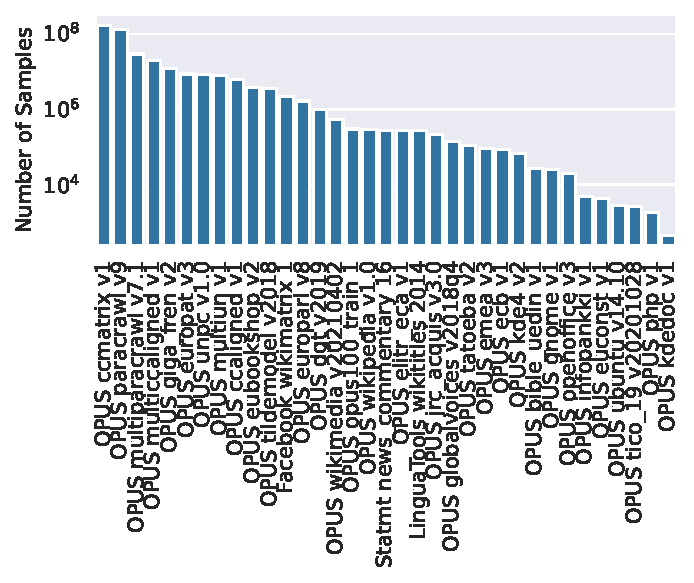
\includegraphics[width=0.8\textwidth]{images/croissant_images/aligned_distrib.pdf}
    \caption[Opus data distribution]{Opus Data Distribution withinn our training dataset}
    \label{fig:opus}
\end{figure}

\subsection{Scaling Law Corpus}
\label{sec:scaling_data}

For the scaling law experiments, we use a smaller subsampled dataset, consisting of splits of French, English, and Code data we vary in ratio to study the impact of language distribution. In total, we train on 50 billion tokens and sample from the following datasets: French \url{https://huggingface.co/datasets/manu/french-30b}, English \url{https://huggingface.co/datasets/manu/english-60b} and Code \url{https://huggingface.co/datasets/manu/code_20b}. In all datasets, a breakdown of the sources is given in the \textit{dataset\_stats.csv} file at the root of the data folder. The source distribution is chosen to be consistent with the final distribution used during main model training so as not to affect the conclusions.

\clearpage
\section{Chat examples}

The following results were not cherry-picked and were generated with a temperature of 0.5, a Top-P of 0.95 and a Top-K of 40. They focus on Writing tasks which CroissantLLM is best at.

\subsection{Translate the following article in French:}

\textit{The Principality of Sealand (/silænd/) is an unrecognised micronation on HM Fort Roughs (also known as Roughs Tower),[5] an offshore platform in the North Sea approximately twelve kilometres (6+1⁄2 nautical miles) off the coast of Suffolk, England.[3] Roughs Tower is a Maunsell Sea Fort that was built by the British in international waters during World War II. Since 1967, the decommissioned Roughs Tower has been occupied and claimed as a sovereign state by the family and associates of Paddy Roy Bates. Bates seized Roughs Tower from a group of pirate radio broadcasters in 1967 with the intention of setting up his own station there. Bates and his associates have repelled incursions from vessels from rival pirate radio stations and the U.K.'s royal navy using firearms and petrol bombs.[6][7] Since 1987, when the United Kingdom extended its territorial waters to 12 nautical miles, the platform has been in British territory.}


 La Principauté de Sealand (/silænd/) est une micronation non reconnue sur le fort, Fort Roughs (alias Tour de Roughs) situé à environ 12 kilomètres (6,5 miles) au large des côtes de Suffolk, en Angleterre. Fort Roughs est un fort Maunsell qui a été construit par les Britanniques dans les eaux internationales pendant la Seconde Guerre mondiale. Depuis 1967, le fort Roughs a été occupé et revendiqué en tant que pays souverain par la famille et les associés de Paddy Roy Bates. Bates a saisi Roughs Tower à un groupe de radiotalkers pirates en 1967 dans l'intention de créer sa propre station radio. Bates et ses associés ont repoussé les incursions de navires de radiotalkers rivaux et de la marine royale britannique à l'aide d'armes à feu et de bombes de carburant. Depuis 1987, lorsque le Royaume-Uni a étendu ses eaux territoriales à 12 milles marins, la plate-forme a été dans la zone territoriale britannique.


\subsection{What can I do in Marseille during the winter ?}

 1. Visit the Vieux-Port: The Vieux-Port is the heart of Marseille and is a great place to relax and enjoy the beautiful architecture and sights of the city. You can also take a boat tour to see the island of the Frioul.

2. Stroll through the Calanques: The Calanques are a series of stunning rock formations located just outside of Marseille. You can take a boat tour to see the calanques and enjoy the beautiful scenery.

3. Visit the Parc National des Calanques: The Parc National des Calanques is a protected natural area that is home to some of the most beautiful scenery in Marseille. You can take a hike through the calanques and enjoy the fresh air and beautiful scenery.

4. Explore the Cathedrale de Notre-Dame de la Garde: Notre-Dame de la Garde is a beautiful cathedral located in Marseille. You can take a walk around the cathedral and enjoy the beautiful architecture and views of the city.

5. Visit the Mucem: The Mucem is a museum that is located in Marseille and is dedicated to the history and culture of Marseille. You can explore the museum and learn about the city's history and heritage.


\subsection{Rédige une lettre de motivation pour un job étudiant de barman.}

 Objet : Candidature pour un job étudiant de barman

Cher [nom du recruteur],

Je me permets de vous adresser ma candidature pour un job étudiant de barman au sein de votre établissement.

Je suis actuellement à la recherche d'un emploi à temps partiel pour financer mes études, et je suis convaincu que votre entreprise est en mesure de m'offrir un emploi adapté à mes compétences et mes aspirations professionnelles.

Je suis quelqu'un de dynamique, motivé et souriant. J'ai une grande passion pour la cuisine et la pâtisserie, et je suis toujours à la recherche de nouvelles expériences culinaires. Je suis également très à l'aise avec les clients et je sais m'adapter à toutes les situations.

Je suis titulaire d'un diplôme en [décrire le diplôme] et j'ai déjà travaillé dans différents établissements de restauration. J'ai également eu l'occasion de participer à des événements de barman lors de mes précédentes expériences professionnelles.

Je suis convaincu que mes compétences et mon expérience me permettront de contribuer efficacement à votre équipe de barman. Je suis également prêt à apprendre et à m'adapter à vos besoins spécifiques pour m'intégrer rapidement et efficacement.

Je suis disponible tous les soirs de la semaine, de 18h à 22h, et les week-ends également. Je suis également prêt à me déplacer pour des événements de barman.

Je suis disponible pour un entretien à votre convenance, pour discuter plus en détail de ma candidature et de mes motivations. Je reste à votre disposition pour toute information complémentaire.

Cordialement,

[Votre nom]


\subsection{Show me how to code a Depth First Search in Python}

 I can provide you with the code for a depth-first search in python. Here is the code:

\begin{lstlisting}

def dfs(graph, start):
    visited = set()
    stack = []
    visited.add(start)
    stack.append(start)

    while stack:
        vertex = stack.pop()
        visited.add(vertex)

        for neighbor in graph[vertex]:
            if neighbor not in visited:
                stack.append(neighbor)
\end{lstlisting}

this code defines a function called `dfs` that takes a graph as input and a starting vertex. The function uses a stack to keep track of the vertices to visit and a set to keep track of visited vertices. The vertices are added to the stack. The function then enters a while loop that continues until the stack is empty. Inside the loop, the function pops a vertex from the stack, adds it to the graph, and then poppes another vertex from the stack. This process continues until all vertices have been visited. Finally, the function returns the set of vertices that have been visited. You can use this function to perform a depth-first search on a graph.

\subsection{Give me medical advice about how to solve my back issues.}

I don't have a physical body or medical knowledge. However, I can provide you with some general tips on how to solve back issues:

1. Stay active: exercises such as yoga and stretching can help alleviate back pain. Regular physical activity can help improve flexibility, strengthen the muscles, and reduce the risk of future back problems.

2. Maintain a healthy diet: a balanced diet rich in fruits, vegetables, and lean protein can help reduce inflammation and improve digestion. Avoid high-fat and high-sugar foods, which can aggravate back pain.

3. Manage stress: chronic stress can worsen back pain. Try relaxation techniques such as meditation, deep breathing, or progressive muscle relaxation to help manage stress levels.

4. Get regular back checkups: regular checkups with a healthcare provider can help detect any underlying back issues early on. This can help prevent future problems.

5. Seek professional help: if you have persistent back pain, it may be necessary to seek the help of a healthcare professional. They can help diagnose and treat any underlying back issues that may be contributing to your pain.

\clearpage
\section{Results}
\subsection{Methodology}
Base models are evaluated through the LM Evaluation harness framework \sidecite{eval-harness}. For classification tasks, we choose the answer with the largest log likelihood when concatenated with the prompt, as is implemented within the framework.

For generative tasks, we simply generate with the default settings, which is greedy sampling. We acknowledge CroissantLLM works best with higher temperature values but did not want to introduce stochasticity to the evaluation. We also limit each benchmark task to 5000 samples at most, to shorten evaluation time. All evaluations are reproducible through the code at \url{https://github.com/EleutherAI/lm-evaluation-harness}.


% \subsection{Perplexity results}
% \label{sec:ppl}
% Communication with the Pagnol model authors \sidecite{launay2021pagnol}, enabled us to compute CroissantLLM perplexity on the same dataset and in the same conditions as the PagnolXL results shared in the paper. PagnolXL is a 1.5B decoder model, and is reported to obtain a French Treebank \sidecite{abeille2003ftb}\sidenote{\url{http://www.llf.cnrs.fr/en/Gens/Abeille/French-Treebank-fr.php} in its SPMRL instance \sidecite{seddah-etal-2013-overview}} Perplexity value of 16.40 (test set), computed \sidenote{\url{https://huggingface.co/docs/transformers/perplexity}}  with a rolling stride of 512 and a max sequence length of 2048 tokens. CroissantLLM obtains a perplexity value of 10.37, largely outperforming the biggest model in the Pagnol family\sidenote{Note that CroissantLLM and Pagnol tokenizers are different}.

\subsection{MT-Bench}

Turn 1 (Figure \ref{fig:mt_bench_fr_t1}) and Turn 2 (Figure \ref{fig:mt_bench_en2}) results are shown. We notice small models, struggle with reasoning based tasks and contrained generation imposed by Turn 2 prompts. Figures \ref{tab:mt_bench_all_fr} and \ref{tab:mt_bench_all_en} compare our results on small language models to other common bigger models.\sidenote{Results in French for models with sizes over 7B parameters were extracted from \url{https://huggingface.co/datasets/bofenghuang/mt-bench-french} and results in English are from \url{https://huggingface.co/spaces/lmsys/mt-bench/tree/main/data/mt_bench/model_judgment}}

\begin{figure*}
    % First figure
    \centering
    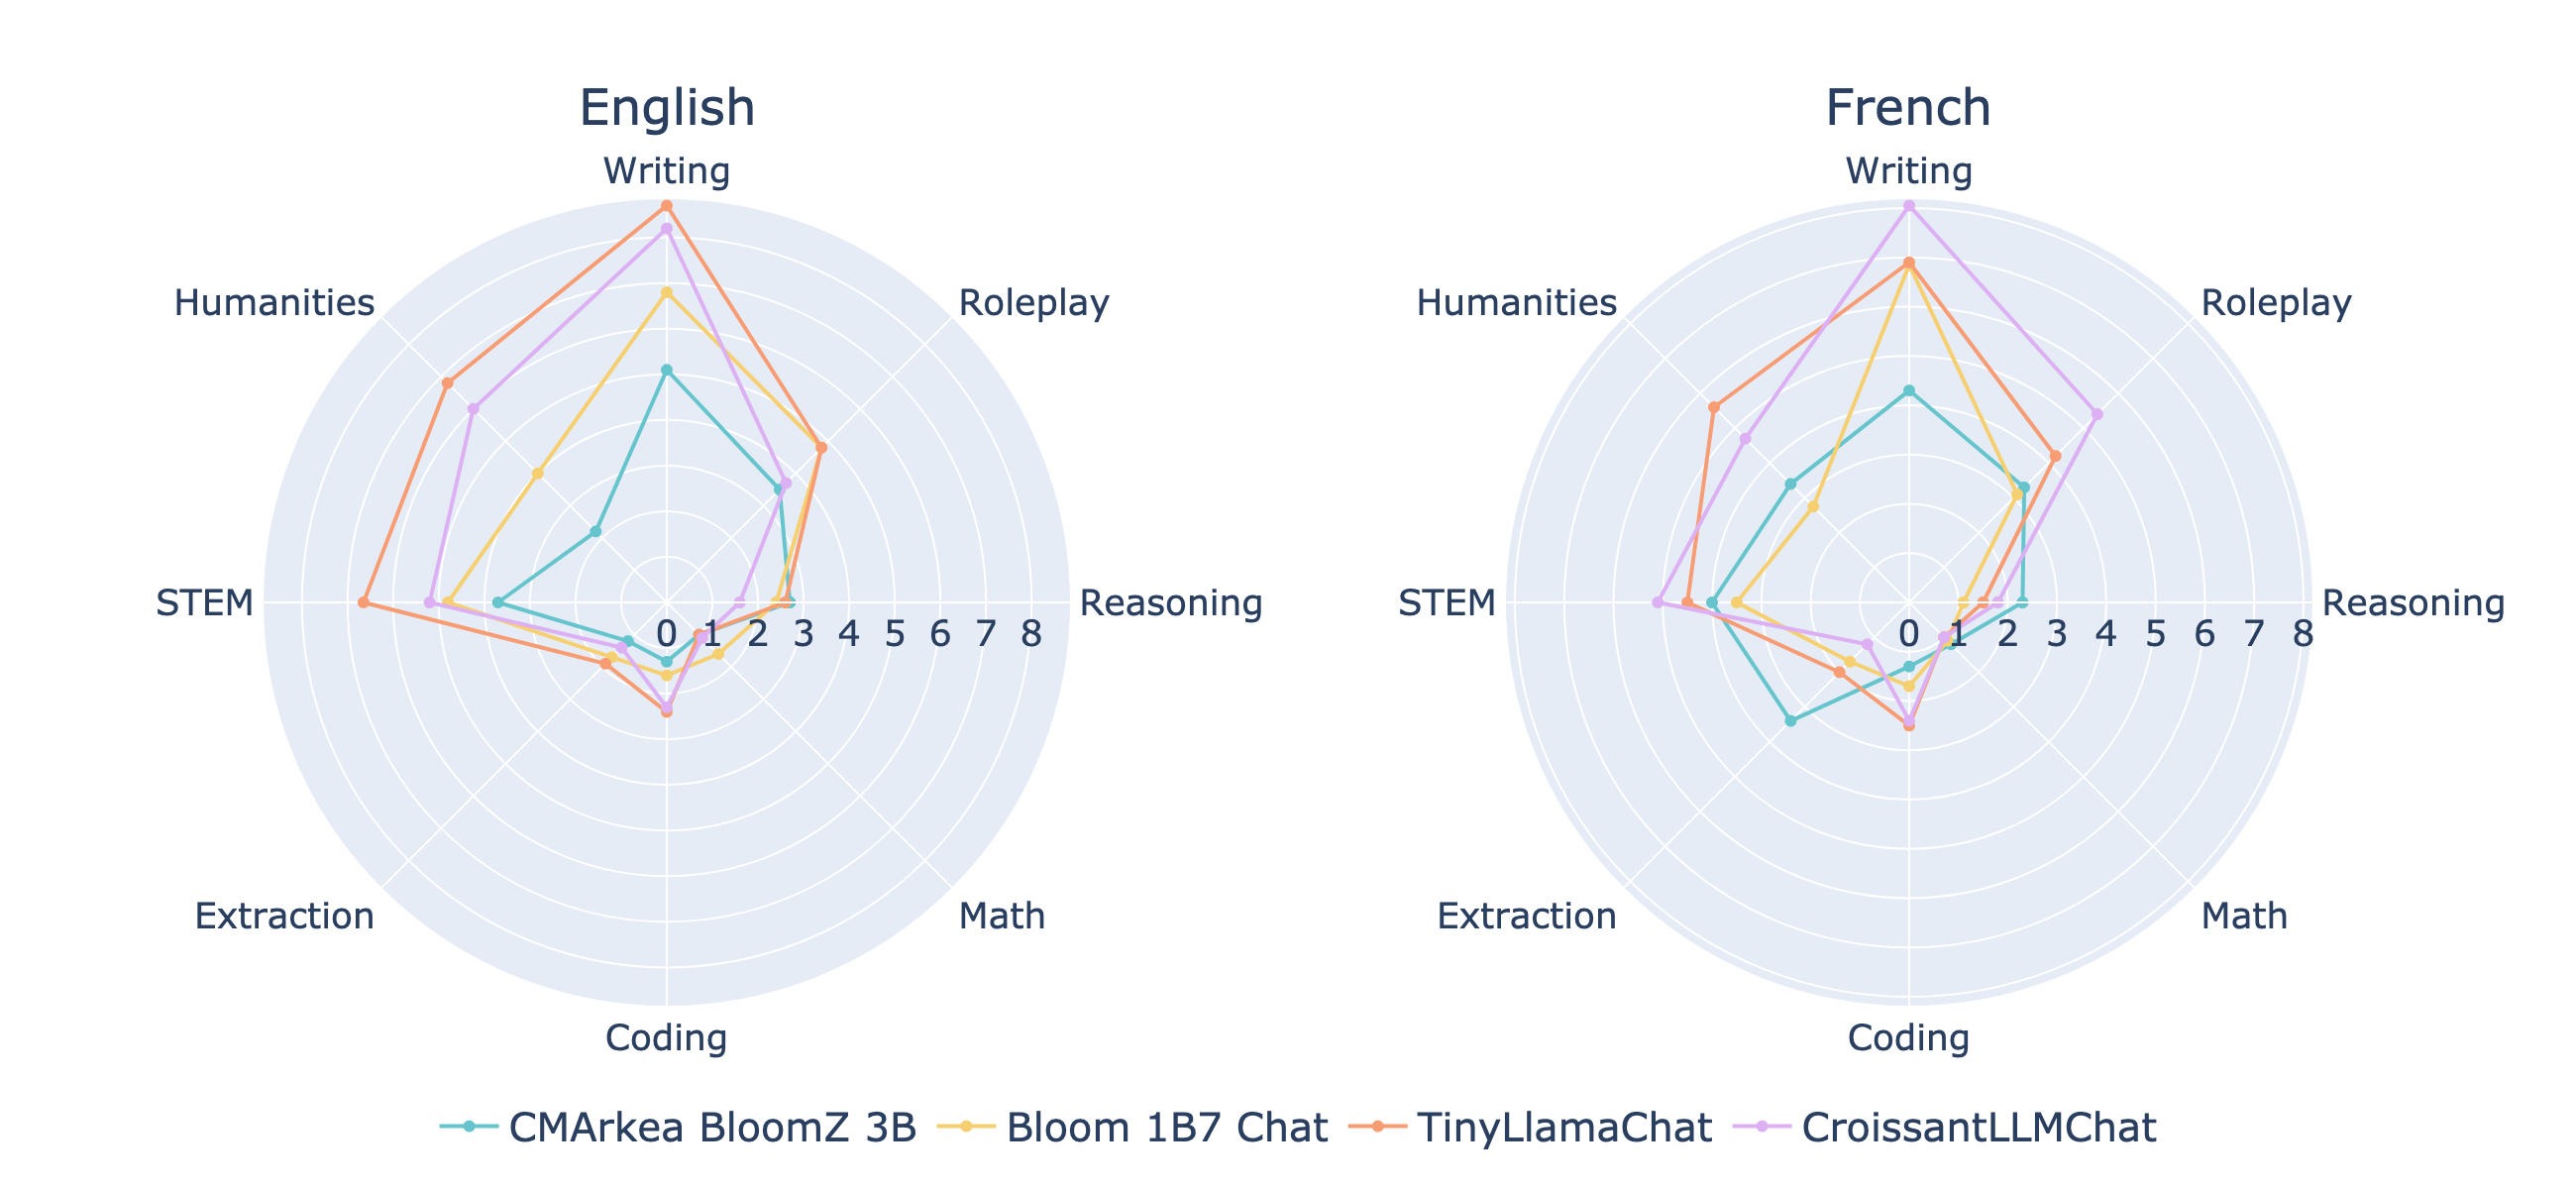
\includegraphics[width=\linewidth]{images/croissant_images/results_turn_1.png}
    \caption[MT Bench results turn 1]{MT Bench Results (Turn 1)}
    \label{fig:mt_bench_fr_t1}
\end{figure*}


\begin{figure*}
    % First figure
    \centering
    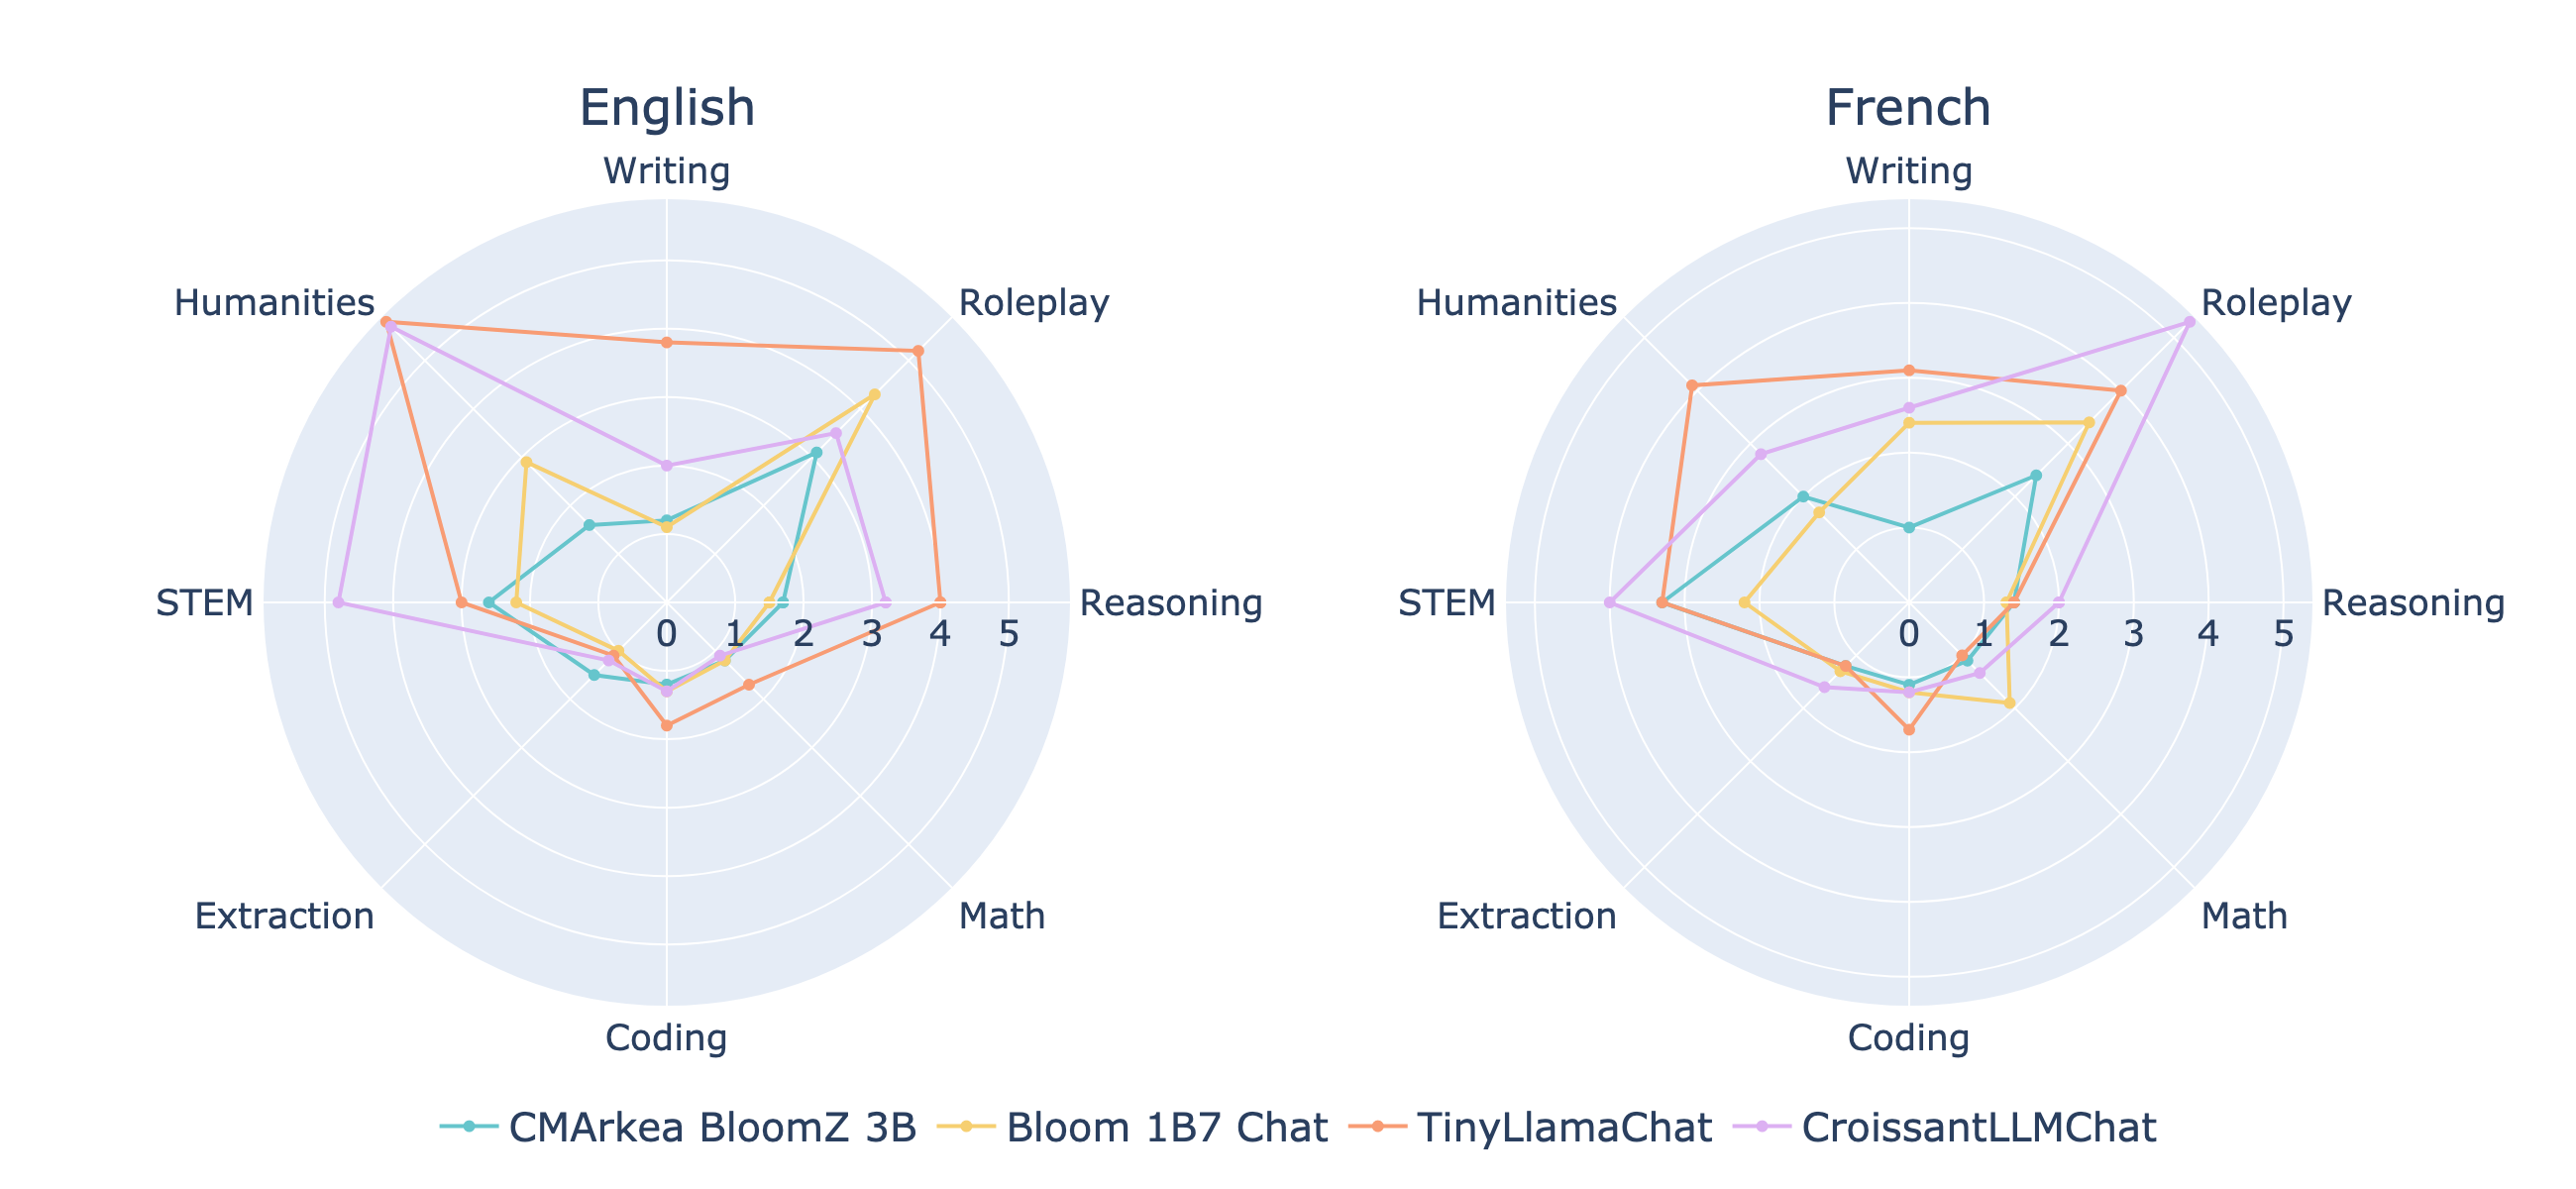
\includegraphics[width=\textwidth]{images/croissant_images/results_turn_2.png}
    \caption[MT Bench results turn 2]{MT Bench Results (Turn 2)}
    \label{fig:mt_bench_en2}
\end{figure*}

\begin{table*}[h]
\centering
\begin{tabular}{lcccccccccc}
\hline
Models & Wri & Ro & Reas & Math & Cod & Ext & STEM & Hum & Avg \\
\hline
CroissantLLMChat & 5.32 & 5.35 & 1.9 & 1.16 & 1.8 & 1.4 & 4.55 & 3.75 & 3.15 \\
TinyLlamaChat & 5 & 4.1 & 1.45 & 1 & 2.1 & 1.6 & 3.9 & 4.85 & 3 \\
Bloom 1B7 Chat & 4.62 & 3.25 & 1.2 & 1.5 & 1.45 & 1.5 & 2.85 & 2.22 & 2.32 \\
CMArkea BloomZ 3B & 2.65 & 2.85 & 1.85 & 1.15 & 1.2 & 2.3 & 3.65 & 2.7 & 2.29 \\
\hline
Vigostral 7B Chat & 7.7 & 7.85 & 4.85 & 3.65 & 4.65 & 7.75 & 7.35 & 9.2 & 6.62 \\
Vigogne 2 7b Chat & 5.35 & 6.25 & 2.75 & 2.2 & 2.47 & 3.4 & 6.05 & 6.68 & 4.39 \\
OpenHermes Mistral 7B & 8.8 & 7.5 & 5.1 & 4.05 & 5.55 & 6.2 & 8.35 & 9.4 & 6.87 \\
Vigogne 2 70B Chat & 9.4 & 8.25 & 4.75 & 4.3 & 5.35 & 7.25 & 9.1 & 9.43 & 7.23 \\
Mixtral 8x7b Instruct & 9.65 & 8.88 & 6.95 & 4.95 & 4.6 & 8.55 & 9.5 & 9.6 & 7.84 \\
Mistral Medium & 9.6 & 9.05 & 5.4 & 6.1 & 7.35 & 9.25 & 9.3 & 9.75 & 8.23 \\
GPT 3.5 Turbo & 8.75 & 8.93 & 5.05 & 5.65 & 7.85 & 9.05 & 9.05 & 9.68 & 8 \\
GPT 4 & 9.6 & 9.65 & 8.55 & 8.5 & 8.35 & 9.2 & 9.85 & 9.88 & 9.2 \\
\hline
\end{tabular}
\caption[French MT Bench average]{French MT Bench Results Average of turn 1 and 2 of many supervised finetuned models}
\label{tab:mt_bench_all_fr}
\end{table*}

\begin{table*}[h]
\centering
\begin{tabular}{lcccccccccc}
\hline
Models & Wri & Ro & Reas & Math & Cod & Ext & STEM & Hum & Avg \\
\hline
CroissantLLMChat      & 5.1     & 3.6      & 2.4       & 1.1  & 1.8   & 1.3        & 5    & 5.85       & 3.27    \\
TinyLlamaChat         & 6.25    & 5        & 3.3       & 1.35 & 2.1   & 1.5        & 4.82 & 6.3        & 3.83    \\
Bloom 1B7 Chat        & 3.95    & 4.55     & 1.95      & 1.4  & 1.45  & 1.35       & 3.5  & 3.45       & 2.7     \\
CMArkea BloomZ 3B     & 3.15    & 3.3      & 2.2       & 1.1  & 1.25  & 1.35       & 3.15 & 1.9       & 2.17    \\
\hline
Llama 2 7B Chat       & 8.9     & 7.7      & 4.25      & 2.4  & 3     & 6.5        & 8.65 & 8.75      & 6.27    \\
Vicuna 7B v1.3        & 8.1     & 7.45     & 4.65      & 2.3  & 3.55  & 5          & 7.82 & 9.1       & 6       \\
Llama 2 13B Chat      & 8.85    & 7.5      & 5.1       & 3.45 & 3     & 6.92       & 8.62 & 9.75      & 6.65    \\
Vicuna 13B v1.3       & 9.25    & 7.18     & 5.85      & 2.6  & 3.25  & 5.55       & 7.98 & 9.45      & 6.39    \\
Vicuna 33B v1.3       & 9.5     & 8.45     & 6.65      & 3.15 & 3.35  & 7.1        & 8.98 & 9.8       & 7.12    \\
Llama 2 70B Chat      & 9.3     & 7.5      & 5.8       & 3.3  & 3.15  & 7.25       & 8.93 & 9.62      & 6.86    \\
GPT 3.5 Turbo         & 9.2     & 8.4      & 5.65      & 6.3  & 6.9   & 8.85       & 8.7  & 9.55      & 7.94    \\
GPT 4                 & 9.65    & 8.9      & 9         & 6.8  & 8.55  & 9.38       & 9.7  & 9.95      & 8.99    \\
\hline
\end{tabular}
\caption[English MT Bench average]{English MT Bench Results Average of turn 1 and 2 of many supervised finetuned models}
\label{tab:mt_bench_all_en}
\end{table*}


\subsection{Bias Assessment}

We assess bias through CROWS \sidecite{nangia2020crowspairs, neveol-etal-2022-french-crows}, the Crowdsourced Stereotype Pairs benchmark that cover stereotypes dealing with nine types of bias, like race, religion, and age and report results in Table~\ref{tab:bias}. We find CroissantLLM is in line, or slightly less biased than other models, notably in French. 

\begin{table}
    \centering
\begin{tabular}{lrrr}
\toprule
    Task & Crows(en) & Crows(Fr) & Avg \\
    \midrule
    mGPT(1.3B) & 3.16 & 2.94 & 3.05 \\
    Bloom(3B) & 3.39 & 3.02 & 3.21 \\
    Bloom(1.1B) & 3.36 & 3.07 & 3.22 \\
    \textbf{CroissantLLM} & 3.56 & 3.22 & 3.39 \\
    Pythia(1.4b) & 3.36 & 3.62 & 3.49 \\
    OPT(1.3b) & 3.35 & 3.67 & 3.51 \\
    TinyLlama(1.1B) & 3.48 & 3.76 & 3.62 \\
    GPT-fr(1B) & 4.50 & 2.97 & 3.73 \\
    Llama2(7B) & 3.72 & 3.81 & 3.76 \\
    \bottomrule
    \end{tabular}

    \caption[Bias evaluation on Crows-Pairs]{Bias Evaluation through Crows-Pairs dataset assessed by likelihood difference.}
    \label{tab:bias}
\end{table}

\subsection{MMLU Results}

The MMLU benchmark \sidecite{hendrycks_measuring_2020} has become standard in evaluating Large Language Model knowledge and reasoning capabilities. However, it is still currently very challenging for smaller models, and even very recent pretrained models such as Llama 3.2(1B) or Gemma2 \sidecite{dubey2024llama3herdmodels, gemmateam2024gemma2improvingopen} report base model performances that are only slightly better than random ($\leq 33\%)$. CroissantLLM, TinyLlama, and other small model baselines in this paper display random performance on the task ($\approx 25\%)$ which is why the task is not included in the main paper.

\clearpage
\section{Terminology}
\label{sec:terminology}

\noindent\textbf{Large Language Models.} 
According to the definition proposed by \sidecite{rogers2024positionkeyclaimsllm}, Large Language Models (LLMs) (1) have the capacity to model and generate text, (2) are pretrained on large amounts of text data (over 1B tokens according to the proposed threshold) (3) enable transfer learning through finetuning or prompting. Under these criteria, CroissantLLM can largely be considered a large language model despite its small size relative to current best-in-class LLMs.

\noindent\textbf{Small Language Models.} Small Language Models (SLMs) is a term that has appeared more recently and that refers to LLMs with a relatively low parameter count, often optimized for speed or to enable inference with local or lower-end hardware.

\noindent\textbf{Effective Capacity Ratio.} Introduced in \sidecite{pmlr-v202-fernandes23a}, the \textit{effective parameters} of a multilingual model in a particular language is the number of non-embedding parameters a monolingual model would require to match the language performance of the multilingual model. The intuition is that a multilingual model splits its capacity between different languages, so a monolingual model would reach similar performances on a specific language with a fraction of the parameters. We further compute the \textit{effective capacity ratio} by dividing the effective parameters by the multilingual model size. In our joint scaling laws experiments (\autoref{fig:scaling-laws-capacity}), we show that the models trained with equal ratios of English to French have an \textit{ effective capacity ratio} of over 82\% in the French language, indicating that training a monolingual French model with the same performance would require about 82\% of the non-embedding parameters. This hints there must be some effective capacity sharing between English and French.


\noindent\textbf{Tokenizer fertility.} According to \sidecite{rust2021good}, \textit{fertility} measures the average number of sub-words (tokens) produced per tokenized word. De facto, fertility has a theoretical lower bound of 1 which would imply that the tokenizer’s vocabulary contains every word in the corpus. 


\clearpage
\section{Post-Mortem \& Lessons learned}
In line with our efforts of full transparency, we share some key lessons learned through this project, in light of a few months of hindsight and of recent developments posterior to the model release.


\noindent\textbf{Tokenizer.} 
In this work, we have developped our own tokenizer, inspired by Llama2 \sidecite{touvron2023llama2} but fitted to a bilingual French-English corpus to improve fertility on both languages. Several key decisions can impact tokenizer design. The \textit{vocabulary size} will have large impacts on the parameter count of the model, potentially making embedding parameters a large share of the total parameter count especially for smaller models \sidecite{gemmateam2024gemma2improvingopen}. One should experiment with the performance and memory trade-offs of using larger vocabulary sizes. Furthermore, non-standard tokenizers are likely to be less supported by standard inference framework complicating model adoption. Finally, we believe hand-designing a subset of tokens that are known to be useful at inference, for particular tasks, or have semantic coherence (common numbers, punctuation patterns, tokens corresponding to multiple choice templates or code syntax) probably degrades fertility but is useful in the long run from a performance and usability perspective.


\noindent\textbf{Data Mix.} It was always understood the data quality and quantity of the pretraining mix had large impacts on pretraining. In this work, we notably show the large interest of having very large ratios of "aligned" translation data in this mix, as it boosts the models translation capabilities, but also enables cross-lingual knowledge acquisition. 
Since CroissantLLM's release, it has become understood that certain types of data heavily boost model reasoning capalities or performances on benchmarks.
Typically, \sidecite{abdin2024phi3technicalreporthighly, rekateam2024rekacoreflashedge, yang2024qwen2technicalreport, dubey2024llama3herdmodels},  put a particular emphasis in including math and reasoning heavy corpora in the training corpus. \sidecite{Groeneveld2023OLMo} reports 24 point gains on MMLU scores by including more knowledge and reasoning rich sources to their training set, as well as improving data quality filtering. In order to source such data with highly "educative" values several approaches are possible, including distilling large model knowledge into fast text classifiers to identify high-quality content from Internet scale data \sidecite{penedo2023refinedweb}, or even generating diverse and high quality synthetic text using LLMs \sidecite{abdin2024phi3technicalreporthighly, benallal2024cosmopedia, dubey2024llama3herdmodels}. More generally, better pretraining and annealing data leads to better models, and many recent datasets would probably lead to better performance nowadays than the datamix we had constituted. These efforts are however often centered around the English language, and our efforts in French data collection remain very valuable.
% translations
% math and reasoning
% synthetic data

\noindent\textbf{Scheduler.} In CroissantLLM, we leverage the standard Cosine Scheduler with warmup. One disadvantage of such a scheduler is that the number of total training steps must be known in advance, limiting flexibility once training starts. Inspired by the Vision literature \sidecite{zhai2022scalingvisiontransformers}, the MiniCPM model \sidecite{hu2024minicpmunveilingpotentialsmall} and several models since then have later confirmed the interest of infinite or WSD (Warmup-Stable-Decay) schedulers\sidecite{hägele2024scalinglawscomputeoptimaltraining}. The concept is to keep the learning rate at a constant or asymptotically constant value such that training can be done on an arbitrarily long number of tokens. At the end of training, an \textit{annealing} phase decreases the learning rate to help the model converge and boost performance. MiniCPM has further uncovered that annealing on a higher quality data mix is a very efficient strategy. Typically, by including knowledge-rich or reasoning-heavy data in this final training phase, large benchmark improvements are obtained. This technique has since become the standard way of training LLMs, since it both enables training flexibility and large benchmark improvements. We believe running an annealing phase on the CroissantLLM model would have largely boosted performance, especially if done with carefully selected high-quality data in French and English.

\noindent\textbf{Leveraging Larger LLMs.} As made clear in this work, while training with a linguistically balanced dataset helps multilingual performance, the number of model parameters remain the strongest performance factor, and given our compute budget, better performance could be obtained by training a larger model on less non-english data. This is perfectly in line with the findings of \sidecite{kaplan2020scaling} with Chinchilla scaling laws. Models trained to be small and inference efficient such as CroissantLLM could however benefit from larger multilingual LLMs in multiple ways. Beyond the evergrowing use of LLM-generated data during pretraining \sidecite{abdin2024phi3technicalreporthighly}, small models can also benefit from larger LLMs as critics for alignement processes \sidecite{yang2024qwen2technicalreport}, but also to replace stochastic weight initialization by starting off from pruned-versions of larger models \sidecite{dubey2024llama3herdmodels}. Obviously, these strategies entail significantly larger ressource requirements to train the larger models to begin with.


\noindent\textbf{Model Release.} Training a model is one thing, enabling people to use it is another. Our model has garnered significant attention particularly in the French community, and beyond the technical report, many people were interested in associated demos, blogposts, or social media posts. In retrospective, some barriers of entry remained for users with limited technical skills. The lack of day 0 support from third party inference libraries (Ollama\sidenote{\url{https://ollama.com/}}, llama.cpp\sidenote{\url{https://github.com/ggerganov/llama.cpp}}, MLCChat\sidenote{\url{https://llm.mlc.ai/}})has led to some community-proposed implementations that were suboptimal, leading to performance hits. Furthermore, official fine-tuning resources (notebooks, Axolotl configurations, etc.) could have largely helped users adapt CroissantLLM for specific use cases and drive adoption. Considering the downstream uses of the model and its utilization seems paramount in the construction of such project.


\noindent\textbf{Building a model is an iterative process.} Building upon the CroissantLLM work and the above listed insights, our team has since been able to train stronger models \sidecite{martins2024eurollmmultilinguallanguagemodels, boizard2025eurobertscalingmultilingualencoders}. The field evolves quickly and getting everything right the first time is not easy. To build very good models, it seems important to us to construct the foundations iteratively, getting things to work at a small scale first, collecting some practical real-world feedback and keeping a core model development team stable.
